Lai gan detalizēti modeļi ļauj ģenerēt signālus, kas cieši līdzinās īstu neironu signāliem, šādu neironu tīklu realizācija un analīze ir sarežģīta to kompleksās uzvedības dēļ. Lai atvieglotu impulsu kodēšanas un izplatīšanās izpēti neironu tīklos, izstrādāti formāli impulsu ģenerēšanas modeļi. Vēsturiski visplašāk izmantotie formālie modeļi ir Lapika \cite{abbott1999} un Steina \cite{stein1967} izstrādātie \Gls{if} un \Gls{lif} modeļi. Abus modeļus bieži realizē aparatūrā.

Lapika modelētais \Gls{if} neirons sastāv no elektriskās ķēdes ar kondensatoru, kas reprezentē membrānas kapacitāti un uzkrāj ieejas strāvu, līdz tiek sasniegts impulsu ģenerēšanas slieksnis. \Gls{lif} modelis to paplašina, pievienojot paralēli membrānas kapacitātei pieslēgtu membrānas noplūdes rezistoru, izveidojot \ref{fig:lif_circuit}. attēlā parādīto ekvivalento RC ķēdi. Kad membrānas potenciāls sasniedz noteiktu slieksni, tiek ģenerēts darbības potenciāls un kondensators izlādējas. Lai gan dažādu membrānas vadītspēju ietekme netiek ņemta vērā, daudziem mērķiem pietiek ar vienkāršo \Gls{if} modeli.

\begin{figure}[hb]
  \centering
  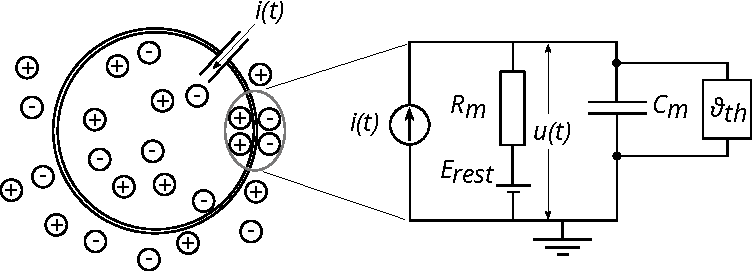
\includegraphics[width=1.0\linewidth]{fig/lif_circuit_membrane.pdf}
  \caption{Integrējošā impulsu neirona modelis ar noplūdi. Šūnas membrāna saņem ieejas strāvu $i(t)$, kas palielina membrānas lādiņu.}
  \label{fig:lif_circuit}
\end{figure}

\Gls{lif} modelī strāva \(i(t)\) uzlādē RC ķēdi, līdz spriegums uz kondensatora \(C_m\) sasniedz noteiktu sliekšņa vērtību \(\vartheta_{th}\). Šajā ķēdē strāva \(i(t)\) sadalās strāvā \(i_C\), kas plūst caur kondensatoru, un strāvā \(i_R\), kas raksturo viena membrānas kanāla pretestību \cite{kim2020}:
\begin{equation}
    i(t) = i_R + i_C = \frac{u(t) - E_{rest}}{R_m} + C_m\frac{du}{dt},
    \label{eq:LIF_current}
\end{equation}
kur \(C_m\) apzīmē membrānas kapacitāti un \(R_m\) ir vienkāršotā kanāla pretestība. Apzīmējot membrānas laika konstanti ar \(\tau_m = R_mC_m\), no (\ref{eq:LIF_current}) iegūst laikā mainīgo membrānas potenciālu, ko rada impulsu strāvas \(i(t)\), kuras caur sinaptiskajiem savienojumiem saņemtas no citiem neironiem:
\begin{equation}
    \tau_m \frac{du}{dt} = - (u(t) - E_{rest}) + R_mi(t),
    \label{eq:LIF_model}
\end{equation}
kur \(i(t)\) ir no atsevišķām sinapsēm saņemto individuālo sinaptisko strāvu summa, katru reizinot ar atbilstošo sinaptiskā svara koeficientu:
\begin{equation}
    i(t) = \sum_{j=1}^{N_{pre}} w_{j}i_j(t),
\end{equation}
kur \(N_{pre}\) ir presinaptisko neironu skaits. Modelis vienkāršojas līdz \Gls{if} neironam, ja membrānas pretestībai piešķir lielu vērtību \(R_m \to \infty\).

Kad membrānas potenciāls sasniedz impulsu ģenerēšanas slieksni, \Gls{lif} neirons izstaro impulsu un pārraida to nākamajiem neironiem. Neirona izejas signāls ir Diraka delta funkcijas impulss \(\delta(t - t^f)\), kur laiku \(t^f\) iegūst, salīdzinot membrānas potenciālu \(u(t^f)\) ar sliekšņa vērtību \(\vartheta_{th}\):
\begin{equation}
    t^f: u(t^f) = \vartheta_{th}
\end{equation}
Matemātiski šādu impulsu notikumu virkni var aprakstīt šādi \cite{kim2020}:
\begin{equation}
    s(t) = \sum_f \delta(t - t^f)
\end{equation}

Impulsa brīdī potenciāls atgriežas nullē vai miera stāvoklī \(E_{rest}\), kas kalpo par sākuma nosacījumu nākamajai aprēķinu iterācijai. Alternatīvi membrānas potenciālu var samazināt par impulsu ģenerēšanas slieksni \(\vartheta_{th}\), veicot mīksto atiestatīšanu, kas precīzāk atdarina \Gls{relu} funkciju \cite{hwang2024, park2019}.

Ja sinaptiskā strāva ir nulle \(i(t) = 0\), membrānas potenciāla vienādojums (\ref{eq:LIF_model}) vienkāršojas līdz
\begin{equation}
    \tau_m \frac{du}{dt} = - (u(t) - E_{rest}).
\end{equation}
Analītiskais atrisinājums ir
\begin{equation}
    u(t) = E_{rest} + (u(t_0) - E_{rest}) \exp \left ( - \frac{t - t_0}{\tau_m} \right ).
    \label{eq:LIF_exp}
\end{equation}
Tas parāda, ka membrānas potenciāls eksponenciāli samazinās līdz miera potenciālam \(E_{rest}\) ar laika konstanti \(\tau_m\).

Vienādojums (\ref{eq:LIF_exp}) apraksta precīzu membrānas potenciālu nepārtrauktā laikā. Tomēr digitālā aparatūra veic diskrēta laika atjaunināšanu, nevis risina nepārtrauktus diferenciālvienādojumus. Diskrēta laika \Gls{snn} simulācijās eksponenciālās dilšanas tiešai novērtēšanai katrā laika solī būtu jāaprēķina:
\begin{equation}
    \exp \left ( \frac{-\Delta t}{\tau_m} \right ).
\end{equation}
Liela mēroga \Gls{snn} ar miljoniem neironu un daudziem laika soļiem tas rada lielu skaitļošanas sarežģītību. Tā kā eksponenciālās operācijas nav izdevīgas digitālo shēmu realizācijās, parasti priekšroku dod aproksimācijai ar bitu nobīdes operācijām vai skaitliskiem atrisinājumiem \cite{corradi2021}. Lielākā daļa \Gls{snn} aparatūras realizāciju diferenciālvienādojumu aproksimē ar vienkāršām skaitliskās integrēšanas metodēm, piemēram, tiešo Eilera metodi, kas eksponenciālās funkcijas aprēķinu aizstāj ar rekurentu vienādojumu.

\ref{fig:lif_simulation}. attēlā parādīta skaitliski atrisināta \Gls{if} modeļa simulācija, tam pievadot konstantas strāvas pakāpienu. Pēc stimula pievadīšanas \(u(t)\) pieaug sliekšņa \(\vartheta_{th}\) virzienā saskaņā ar (\ref{eq:LIF_current}) un, to sasniedzot, izstaro impulsu. Šī vienkāršā uzvedība bez kanālu vadītspējas ilustrē, kādēļ \Gls{if} modelis ir skaitļošanas ziņā izdevīgs, pat neietverot Hodžkina–Hakslija modeļa detalizēto kanālu dinamiku.
\begin{figure}[!t]
\centering
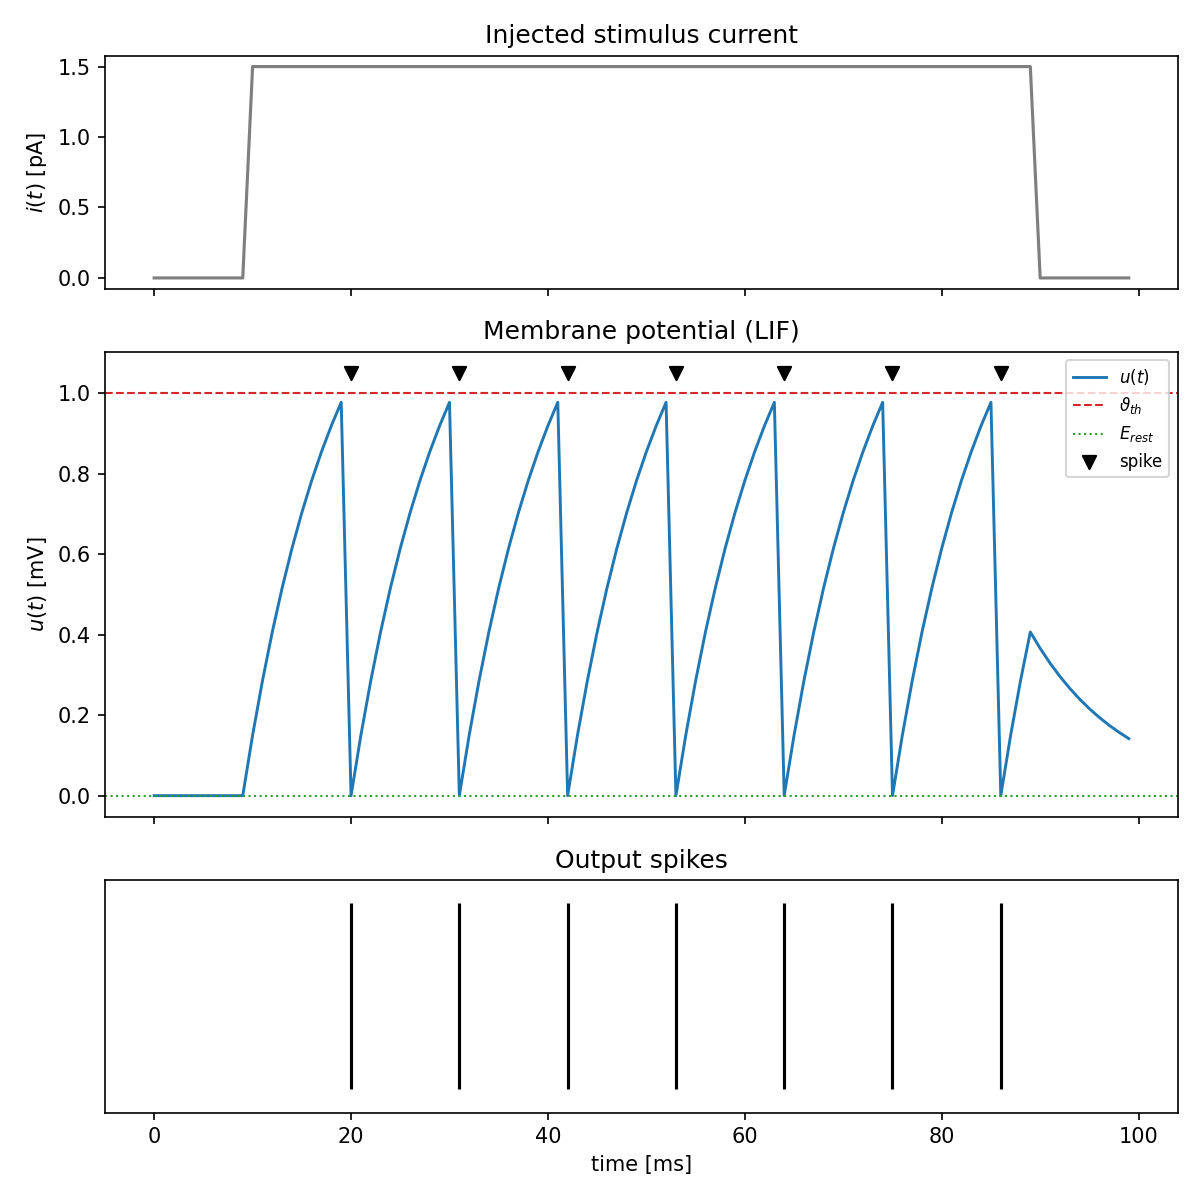
\includegraphics[width=\linewidth]{fig/lif_simulation.png}
\caption{LIF neirona simulētā reakcija uz strāvas pakāpienu.}
\label{fig:lif_simulation}
% \par\smallskip
% {\footnotesize \textit{Injected stimulus current} — pievadītā stimulējošā strāva; \textit{Membrane potential (LIF)}
%   — membrānas potenciāls (LIF); \textit{Output spikes} — izejas impulsi; \textit{spike} — impulss; \textit{time}
%   — laiks.\par}
\end{figure}

Turklāt ir piedāvātas vairākas precizitātes uzlabošanas metodes \Gls{lif} neirona līmenī, lai atvieglotu apmācību un mazinātu
precizitātes zudumu \cite{Fang2021, wang2022, guo2022}. Tiešās izplatīšanas laikā sliekšņa operācija, kas kvantē membrānas
potenciālu līdz 0 vai 1, neizbēgami rada informācijas zudumu. Efektīvs veids, kā mazināt šī vienkāršā modeļa radīto zudumu,
ir padarīt dažus ar membrānu saistītos hiperparametrus apmācāmus. Nesen darbā \cite{Fang2021} parādīts, ka \Gls{snn} ar
parametriskiem \Gls{lif} neironiem pārspēj modernākās metodes gan statiskajās, gan neiromorfajās datu kopās. Papildus sinapšu
svariem par apmācāmu parametru izmantota membrānas laika konstante. Citos darbos \Gls{snn} mācīšanās spēju uzlabošanai
izmantots impulsu neirons ar adaptīvu slieksni \cite{wang2022}. Darbā \cite{guo2022} sniegts visaptverošs pārskats par
dažādām parametriskām, neirona līmeņa apmācības metodēm.


